%%%%%%%%%%%%%%%%%%%%%%%%%%%%%%%%%%%%%%%%%
% Kieker Monitoring Component
% 
% $Date$
% $Rev$:
% $Author$


\chapter{The \KiekerMonitoringPart{} Component}\label{chap:componentsMonitoring}


\section{Configuration}\label{sec:monitoring:configuration}

\KiekerMonitoringPart{} is being configured by a properties file. A sample %
configuration file, which can be used as a template for custom configurations, %
is provided by the file \file{\monitoringPropertiesFile} in the directory %
\dir{\KiekerDir/META-INF/} of the binary release %
(see Section~\ref{sec:example:downloadInstall}). %
Appendix~\ref{sec:appdx:monitoringproperties} lists this file with a documentation 
of all available properties.

In order to use a custom configuration file, the file location needs to be passed to %
the JVM using the parameter \textit{kieker.monitoring.properties}, as shown in %
Listing~\ref{lst:monitoringPropertiesPassedToJVM}. If no configuration file %
is passed, a default configuration (according to the sample file) is being %
used by \KiekerMonitoringPart{}. %

\setBashListing
\begin{lstlisting}[label=lst:monitoringPropertiesPassedToJVM]
#\lstshellprompt# java	#\textbf{-Dkieker.monitoring.properties=}#<ANY-DIR>/my.kieker.monitoring.properties #[\ldots]#
\end{lstlisting}

\section{Monitoring Controller}\label{sec:componentsMonitoring:monitoringController}

The \class{MonitoringController} constructs and controls a \KiekerMonitoringPart{} %
instance and provides methods to, among others, log monitoring records %
(\method{newMonitoringRecord}) employing the configured monitoring log writer and %
to retrieve the current timestamp (\method{currentTimeNanos}). %
The class is implemented employing the singleton pattern. The singleton instance %
can be retrieved by calling the static method \method{getInstance}. %
Figure~\ref{fig:monitoringController:classdiagram} shows %
a class diagram of the class \class{MonitoringController} including the methods 
just mentioned. The \class{MonitoringController} is configured based on a configuration %
file, as described in Section~\ref{sec:monitoring:configuration}.


\begin{figure}[H]\centering
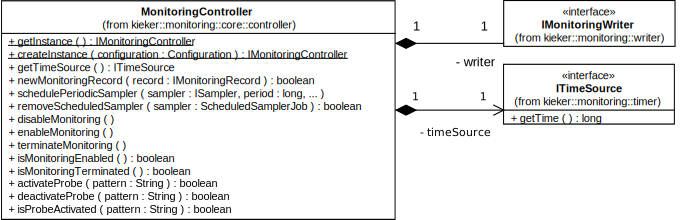
\includegraphics[width=0.95\textwidth]{images/kieker_monitoringControlleruserguide-simplified}
\caption{Class diagram of the \class{MonitoringController} (including selected methods)}
\label{fig:monitoringController:classdiagram}
\end{figure}


\section{Monitoring Records}\label{sec:componentsMonitoring:monitoringRecords}

As mentioned in the previous chapters, monitoring records are the objects that %
contain the monitoring data. Typically, an instance of a monitoring record is %
constructed in a monitoring probe (Section~\ref{sec:monitoring:probe}), %
passed to the monitoring controller (Section~\ref{sec:componentsMonitoring:monitoringController}), %
serialized and deserialized by monitoring a %
monitoring log writer (Section~\ref{sec:monitoring-log-writers}) and a
monitoring log reader (sec:analysis:writer) and provided to the %
analyis plugins (Section~\ref{sec:analysis:consumer}) %
by the analyis controller (Section~\ref{sec:analysis:controller}). %
Figure~\ref{fig:KiekerCommunicationDiagram} illustrates this life cycle of a monitoring %
record. %

In Chapter~\ref{chap:example}, we've already introduced and used the monitoring %
record type \class{OperationExecutionRecord}. \Kieker{} allows to use custom %
monitoring record types. Corresponding classes must implement the %
Interface \class{IMonitoringRecord}, shown in Figure~\ref:{todo}. %

\KiekerMonitoringPart{} provides the abstract class \class{AbstractMonitoringRecord} %
which eases the implementation of own record types. 



To implement your own record type, the easiest way is to extend the already existing abstract class \class{kieker.common.record.AbstractMonitoringRecord}. A custom record type must override methods to serialize and deserialize the record data to/from an array. Due to the fact that the data has to be read again, the records have to provide methods to restore the content from an array as well. Listing \ref{listing:MyRecord} shows a simple record implementation which stores information about the called class and method.

\setJavaCodeListing
\lstinputlisting[caption=MyRecord.java, label=listing:MyRecord]{\customComponentsBookstoreApplicationDir/src/bookstoreTracing/MyRecord.java}


\section{Monitoring Probes}\label{sec:monitoring:probe}

The probes are responsible for the monitoring itself. They decide which (and where) information should be collected. Technically, they were already used in the example chapter by manually surrounding the method calls with code to measure the data of interest, %
construct and initialize the monitoring records, as well as to deliver these records to the monitoring controller. %
The code used to manually instrument the method call in the Bookstore example is %
shown in Listing~\ref{listing:cuttingBookstore}. %

		\TODO{avh: use \texttt{MyRecord}}

		% Make sure that this listing will be modified, once the sourcecode changes!!!
		% It must show the whole monitoring of the bookstorecall, from getting the first time to persisting of the record!!
		\lstinputlisting[firstline=15, lastline=24, firstnumber=15, caption=Excerpt from Bookstore.java, label=listing:cuttingBookstore]{\manualInstrumentedBookstoreApplicationDir/src/bookstoreApplication/Bookstore.java}

		\noindent Other specific probes could for example record only the amount of delivered bytes between methods or record only every second method call as well. The possibility to use annotations to make the monitoring much more comfortable will be shown in the appendix.

\section{Monitoring Log Writers}\label{sec:monitoring-log-writers}

		The so called monitoring log writers serialize and persist the recorded informations into files, databases etc. %
%In other words: They get an instance of an \class{IMonitoringRecord} and produce and output of any nature whatsoever.
		Some writers are already implemented, as can be seen in their hierarchy in Figure \ref{figure:monitoringLogWritersHierarchy}.

		% This is the diagram with the hierarchy of the writers.
		\begin{figure}[H]
			\begin{centering}
				\includegraphics[width=0.5\textwidth]{images/kieker_writerimpls}
				\caption{The inheritance hierarchy of the current implemented monitoring log writers}
				\label{figure:monitoringLogWritersHierarchy}
			\end{centering}
		\end{figure}


		\noindent As the example chapter already showed it, each monitoring record is sent to the \class{MonitoringController} which itself calls the current writer. The writer uses the \method{toArray()} method of the record to get the stored information from the record as handable array. The writer writes these objects for example into a CSV file.\\
		The implementation of an own writer is quite simple and can be done by implementing the interface \class{kieker.monitoring.writer.IMonitoringLogWriter}. Listing \ref{listing:MyWriter} shows an example writer which uses a named pipe to write the given records directly into the memory. The class \class{MyPipe} is descriped in the appendix of the tutorial. 

		\setJavaCodeListing
		\lstinputlisting[caption=MyWriter.java, label=listing:MyWriter]{\customComponentsBookstoreApplicationDir/src/bookstoreTracing/MyWriter.java}

		\noindent Making sure that \Kieker\  uses the new writer is done by modifying the above mentioned configuration file \dir{\monitoringPropertiesFile}.

		\setBashListing       
		\begin{lstlisting}
			monitoringDataWriter=bookstoreTracing.MyWriter
			monitoringDataWriterInitString=somePipe
		\end{lstlisting}

		\noindent The first property decides which writer should be used. If none of the already implemented writers is used, the whole name of the class of the writer has to be delivered. The second property is an init string which can be used to initialize the writer in any way. In this case the parameter is used to tell the writer the name of the pipe to be used.\\
		\WARNBOX{ It is important that every implemented writer class has a corresponding reader class, so that the persisted data can be loaded again.}
